% Creating a simple Title Page in Beamer
\documentclass{beamer}
%\usepackage{parskip}
\usepackage{booktabs}
\usepackage[normalem]{ulem}
\useunder{\uline}{\ul}{}
\setlength{\parskip}{\baselineskip} 

% Theme choice:
\usetheme{Madrid}
% Title page details: 
\title[Distal Acupuncture]{Distal Acupuncture: Theory and Practice}
\subtitle{A systems based approach to complex patterns}
\author{Steven Malins, DOM}
\institute{New Mexico Society for Acupuncture and Asian Medicine}
\date{15 September, 2024}
\begin{document}
% Title page frame
\begin{frame}
    \titlepage
\end{frame}

% Outline frame
\begin{frame}[allowframebreaks]{Outline}
    \tableofcontents[hideallsubsections]
\end{frame}



%%%%%% # INTRODUCTION
\section{Introduction}

\begin{frame}{Steven Malins, DOM}
  \begin{figure}
    \centering
    \includegraphics[width=0.9\textwidth]{img/westie01.jpg}
  \end{figure}
\end{frame}

\begin{frame}{Who am I?} %1.1
  \textbf{\Large My Experience}
  \begin{itemize} \itemsep1em
  \item Licensed for 10 years
  \item Community acupuncture for 3 years, 20+ patients per shift
  \item Community acupuncture for indigenous elders 2x month
  \end{itemize}
\end{frame}

\begin{frame}{References}
  \begin{itemize} \itemsep1em
  \item Deadman, P., Al-Khafaji, M., \& Baker, K. (2007). A manual of acupuncture. Journal of Chinese Medicine.
  \item Kuwahara, T. K. (2003). Traditional Japanese Acupuncture: Fundamentals of Meridian therapy. Paradigm Publications.
  \item O'Connor, J., \& Bensky, D. (1981). Acupuncture: A comprehensive text. Editora Roca.
  \item Tan, T. (2007). Acupuncture 1, 2, 3.
  \end{itemize}
\end{frame}

\begin{frame}{Why Distal Acupuncture?} %1.2
  \begin{center}
    \pause
    \begin{enumerate}
    \item \LARGE Distal acupuncture works!
      \pause
    \item \LARGE Patients with mobility issues
      \pause
    \item \LARGE Wide range of conditions treated
      \pause
    \item \LARGE Systems based, treat patterns not symptoms
    \end{enumerate}
  \end{center}
\end{frame}

\begin{frame}{How does acupuncture work?} %1.3
  \textbf{\Large Endorphin Acupuncture Analgesia (AA)}
  \begin{itemize}
  \item AA Works much better than placebo
    \begin{itemize}
    \item 55\% to 85\% of cases
    \item Morphine ~ 75\% of cases!
    \item Placebo ~ 30\% of cases
    \end{itemize}
  \end{itemize}
  \begin{quote}
    In summary, acupuncture stimulates nerve fibers in the muscle, which send impulses to the spinal cord and activates three centers (spinal cord, midbrain, and hypothalamus-pituitary) to cause analgesia.
  \end{quote}

  Stux, G., \& Pomeranz, B. (2012). Basics of acupuncture. Springer Science \& Business Media. 
  
\end{frame}

\begin{frame}{Ling Shu} %1.4
  \begin{quote}
    When there is a perverse disease with pain which goes along both sides of the backbone to reach the top of the head, and the head nods with heaviness, the eyes are blurred, and loins and spine are stiff and rigid, treat the Leg Major Yang at the point in the middle of the crease of the knee.
  \end{quote}

  Jing-Nuan, W. (Trans.). (2011). Ling Shu: Or the spiritual pivot. The Taoist Center.
\end{frame}

\begin{frame}{Diagnosis} %1.5
  \newtheorem{t1.4}{TCM Diagnosis}
  \begin{t1.4}
    TCM diagnosis, eg ``spleen qi vacuity'' works for herbs but is not useful for acupuncture
  \end{t1.4}

\end{frame}

\begin{frame}{When to use Distal Acupuncture?} %1.6
  \newtheorem{t1.5}{What Can Distal Acupuncture Treat?}
  \begin{t1.5}
    Distal Acupuncture can treat (almost) any pattern/condition!
  \end{t1.5}

  \begin{itemize}
  \item Distal Acupuncture affects cells in Mid-Brain and Pituitary Hypothalamus
  \item All 5 shu points are distal on all 12 meridians
  \item Treating patterns and not symptoms reduces number of needles and increases effectiveness!
  \end{itemize}

\end{frame}

\begin{frame}{When NOT to use Distal Acupuncture} %1.7
  
  \textbf{\Large When to avoid Distal Acupuncture}
  \begin{itemize} \itemsep1.5em
  \item Open wounds near points needed
  \item Chronic pain not responsive to DA
  \item Medical Emergencies!
  \end{itemize}

  \newtheorem{t1.6}{Case Study}
  \begin{t1.6}
    MC: abdominal pain, progressively worse past 24h; rebound tenderness; temperature 100.0
  \end{t1.6}
  
\end{frame}

\begin{frame}{Case Study 0.1} %1.8a
  \textbf{\Large 65F MC: Neck pain}
  
  \textbf{\large Subjective}
  
  \textbf{HPI:} Neck pain started ``a few days ago'' worse with neck flexion; patient describes pain as ``stiff''; radiates to whole head; severity 6 out of 10

  \textbf{\large Objective}
  
  \textbf{P:} vacuous; deep; rapid

  \textbf{PE:} BP 110/76, PR 87, T 99.7; patient is slow to answer questions; otherwise unremarkable

\end{frame}

\begin{frame}{Case Study 0.1} %1.8b
  \newtheorem{dx}{Diagnosis}
  \newtheorem{pln}{Plan}
  \textbf{\Large 65F MC: Neck pain}

  \begin{dx}
    \textbf{Suspected Meningitis!}
  \end{dx}

  \begin{pln}
    Refer to ER for lumbar puncture to confirm or rule out Meningitis
  \end{pln}

\end{frame}
  
\begin{frame}{Discussion}
  \begin{figure}
    \centering
    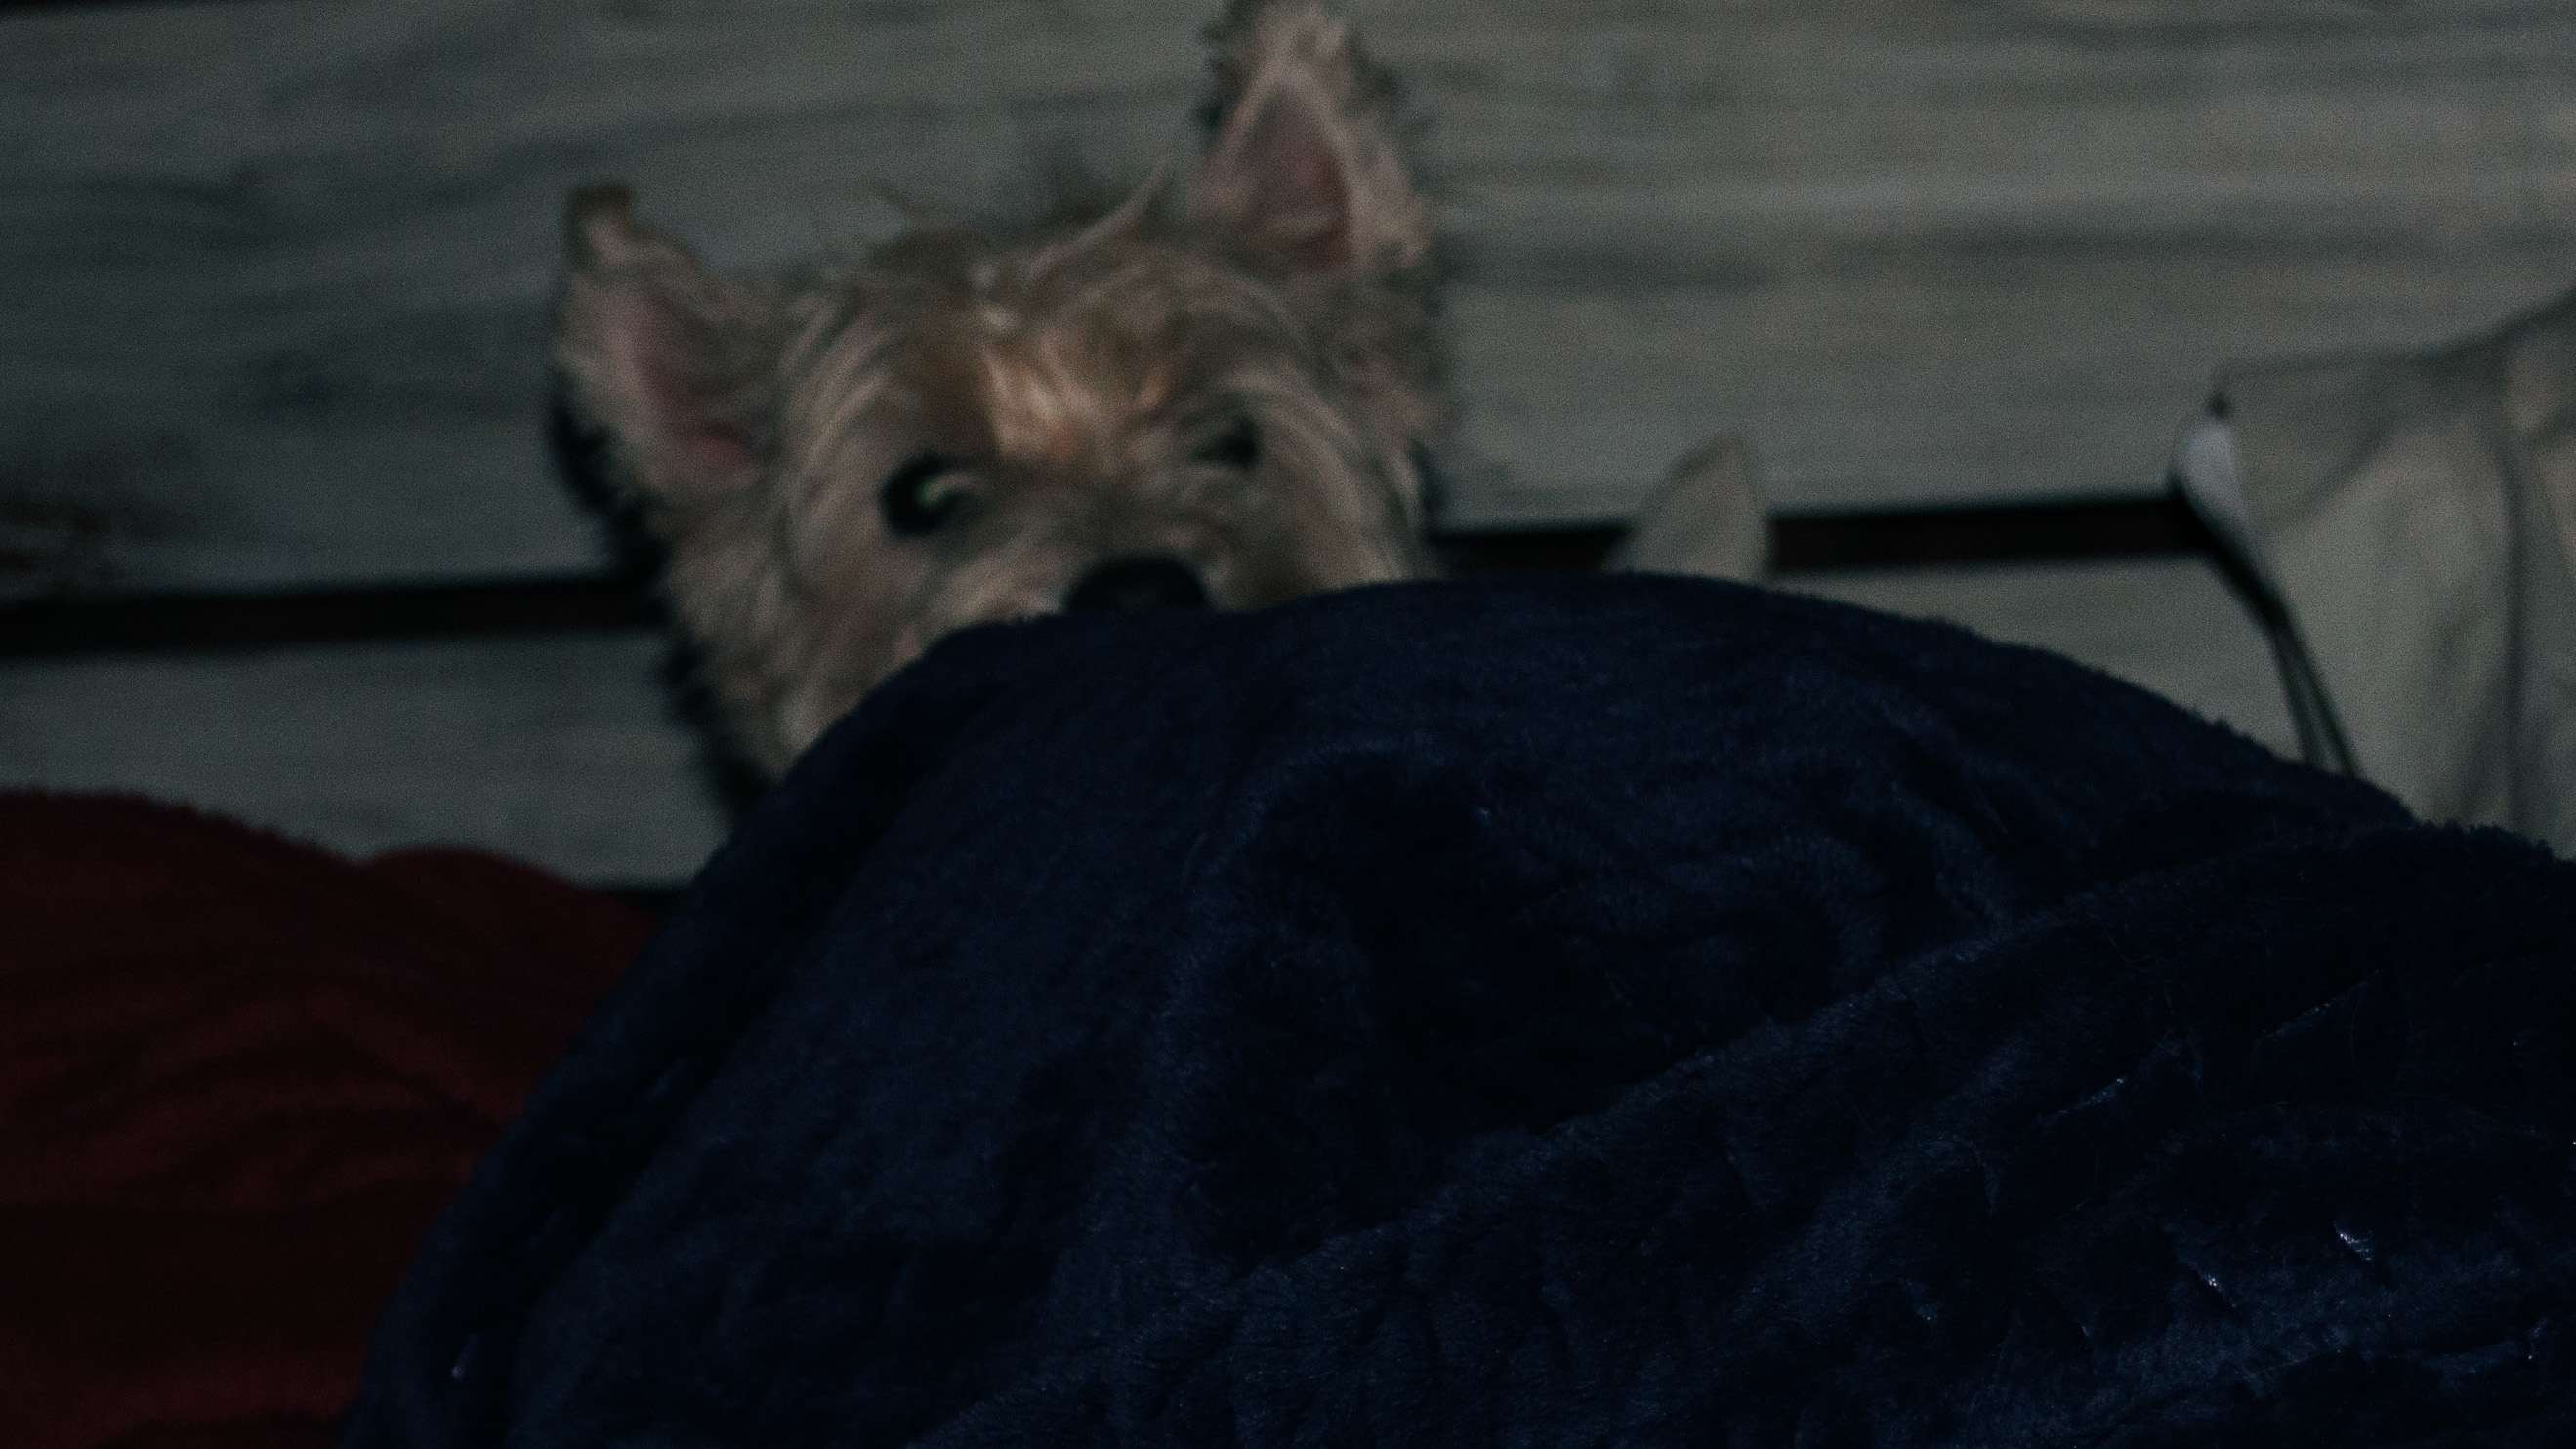
\includegraphics[width=0.9\textwidth]{img/westie02.jpg}
  \end{figure}
\end{frame}

%%%%%% # Miriam Lee
\section{Miriam Lee 10 Points}

%%%%%% # Acupuncture 1,2,3
\section{Acupuncture 1,2,3}

\begin{frame}{Acupuncture 1,2,3}
  \begin{itemize}
  \item Dr Richard Tan
  \item Three Steps:
    \begin{itemize} \itemsep1em
    \item \textbf{Step 1:} Diagnose the Sick Meridian
      \begin{itemize}
      \item Inspection
      \item Auscultation
      \item Inquiry
      \end{itemize}
    \item \textbf{Step 2:} Determine Treating Meridians
      \begin{itemize}
      \item{5 Systems}
      \end{itemize}
    \item \textbf{Step 3:} Point selection
    \end{itemize}
  \end{itemize}

  \begin{quote}
    An affected meridian may indicate soley a physical pain, or may be an indication of an internal issue
  \end{quote}
\end{frame}

\begin{frame}{System I}
  \newtheorem{ns}{Needle Side}
  \textbf{\Large Meridian Name-Sharing}

  \begin{table}[]
    \begin{tabular}{@{}ll@{}}
      \toprule
      Meridian 1                    & Meridian 2                \\ \midrule
      Lung Hand TaiYin              & Spleen Foot TaiYin        \\
      Large Intestine Hand YangMing & Stomach Foot YangMing     \\
      Heart Hand ShaoYin            & Kidney Foot ShaoYin       \\
      Small Intestine Hand TaiYang  & Bladder Foot TaiYang      \\
      Triple Burner Hand ShaoYang   & Gallbladder Foot ShaoYang \\
      Pericardium Hand JueYin       & Liver Foot JueYin         \\ \bottomrule
    \end{tabular}
  \end{table}
  \begin{ns}
    Opposite Side
  \end{ns}
\end{frame}

\begin{frame}{System II}
  \textbf{\Large Branching Meridians}
  \begin{table}[]
    \begin{tabular}{@{}ll@{}}
      \toprule
      Meridian 1                    & Meridian 2                 \\ \midrule
      Lung Hand TaiYin              & Bladder Foot TaiYang       \\
      Large Intestine Hand YangMing & Liver Foot JueYin          \\
      Heart Hand ShaoYin            & Gallbladder  Foot ShaoYang \\
      Small Intestine Hand TaiYang  & Spleen Foot TaiYin         \\
      Triple Burner Hand ShaoYang   & Kidney Foot ShaoYin        \\
      Pericardium Hand JueYin       & Stomach Foot YangMing      \\ \bottomrule
    \end{tabular}
  \end{table}

  \begin{ns}
    Either Side
  \end{ns}
\end{frame}

\begin{frame}{System III}
  \textbf{\Large Interior Exterior}
  \begin{table}[]
    \begin{tabular}{@{}ll@{}}
      \toprule
      Meridian 1  & Meridian 2      \\ \midrule
      Lung        & Large Intestine \\
      Heart       & Small Intestine \\
      Pericardium & Triple Burner   \\
      Spleen      & Stomach         \\
      Kidney      & Bladder         \\
      Liver       & Gallbladder     \\ \bottomrule
    \end{tabular}
  \end{table}

  \begin{ns}
    Opposite Side
  \end{ns}
\end{frame}

\begin{frame}{System IV}
  \textbf{\Large Clock Opposites}

  \begin{figure}
    \centering
    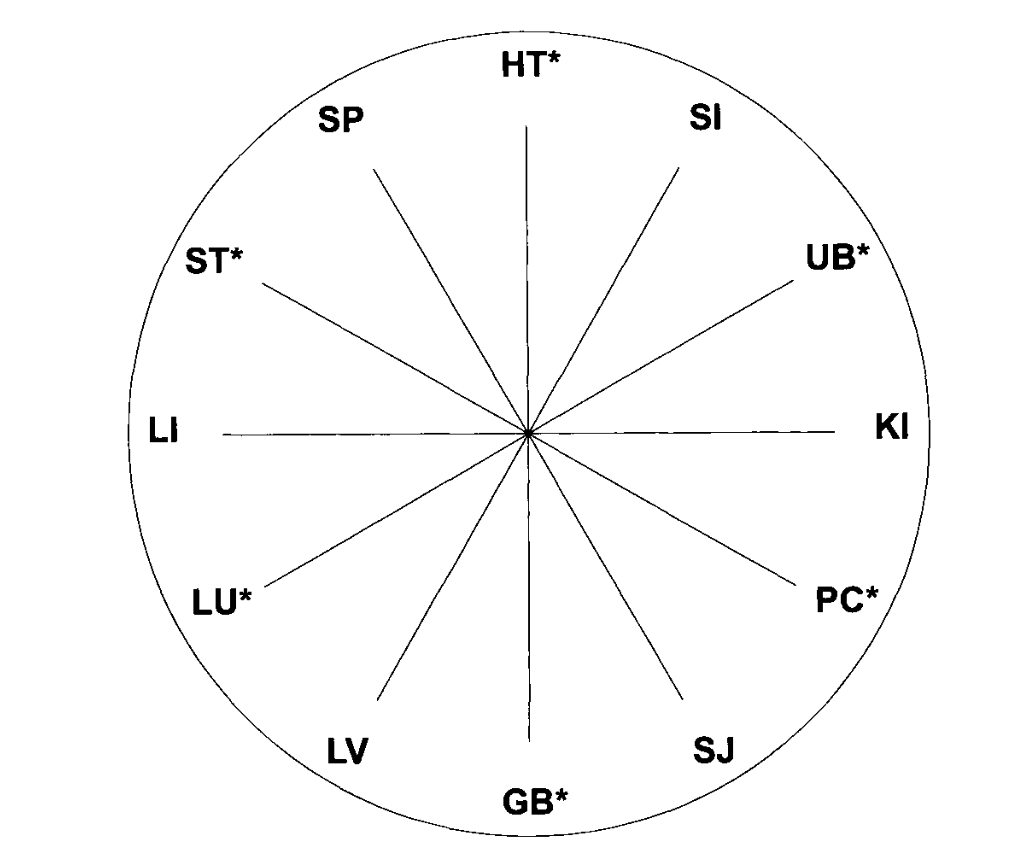
\includegraphics[height=0.5\textheight]{img/mclock.png}
  \end{figure}

  \begin{ns}
    Either Side
  \end{ns}
\end{frame}

\begin{frame}{System V}
  \textbf{\Large Clock Neighbors}

  \begin{table}[]
    \begin{tabular}{@{}ll@{}}
      \toprule
      Meridian 1                        & Meridian 2                    \\ \midrule
      Lung                              & Liver                         \\
      \textit{\textbf{Large Intestine}} & \textit{\textbf{Stomach}}     \\
      Spleen                            & Heart                         \\
      \textit{\textbf{Small Intestine}} & \textit{\textbf{Bladder}}     \\
      Kidney                            & Pericardium                   \\
      \textit{\textbf{Triple Burner}}   & \textit{\textbf{Gallbladder}} \\ \bottomrule
    \end{tabular}
  \end{table}
  
  \begin{ns}
    Opposite Side
  \end{ns}
\end{frame}

\begin{frame}{Imaging I}
  \begin{table}[]
    \begin{tabular}{l|ll}
      {\ul \textbf{Needled Area}} & \multicolumn{2}{c}{{\ul \textbf{Sick Area}}}                                    \\ \hline
      & \multicolumn{1}{c}{\textit{Image}} & \multicolumn{1}{c}{\textit{Reverse Image}} \\
      Finger                      & Genitals anus                      & Top of head                                \\
      Hand                        & Coccyx, sacrum                     & Base of head                               \\
      Wrist                       & Bladder L-S                        & Neck                                       \\
      Forearm                     & Low AB and Back                    & Upper ab and back                          \\
      Elbow                       & Umbilicus, L-2, waist              & Umbilicus, L-2, waist                      \\
      Upper arm                   & Upper ab and back                  & Low AB and Back                            \\
      Shoulder                    & Base of head                       & Coccyx, sacrum                             \\
      Top of shoulder             & Top of head                        & Genitals anus                             
    \end{tabular}
  \end{table}
\end{frame}

\begin{frame}{Imaging II}
  \begin{table}[]
    \begin{tabular}{l|ll}
      {\ul \textbf{Needled Area}} & \multicolumn{2}{c}{{\ul \textbf{Sick Area}}}                                    \\ \hline
      & \multicolumn{1}{c}{\textit{Image}} & \multicolumn{1}{c}{\textit{Reverse Image}} \\
      Toe                         & Genitals anus                      & Top of head                                \\
      Foot                        & Coccyx, sacrum                     & Base of head                               \\
      Ankle                       & Bladder L-S                        & Neck                                       \\
      Lower Leg                   & Low AB and Back                    & Upper ab and back                          \\
      Knee                        & Umbilicus, L-2, waist              & Umbilicus, L-2, waist                      \\
      Upper Leg                   & Upper ab and back                  & Low AB and Back                            \\
      Hip                         & Base of head                       & Coccyx, sacrum                             \\
      Top of Hip                  & Top of head                        & Genitals anus                             
    \end{tabular}
  \end{table}
\end{frame}

\begin{frame}{Acupuncture 1,2,3 Example}
  \newtheorem{s1}{Diagnose the Sick Meridian}
  \newtheorem{s2}{Determine Treating Meridian}
  \newtheorem{s3}{Point Selection}
  \LARGE{Back Pain}

  Area of Discomfort: Paraspinal pain from L3 to L4, left side
\end{frame}
\begin{frame}{1,2,3}
  \begin{s1}
    Bladder meridian, left side
  \end{s1}

  \begin{s2}
    System 1 \& 5: Small Intestine\\
    System 2 \& 4: Lung\\
    System 3: Kidney
  \end{s2}

  \begin{s3}
    SI 7 to SI 8 right side \\
    LU 5 to LU 6 either side \\
    KI 8 to KI 10 right side \\
  \end{s3}
\end{frame}

\begin{frame}{Acupuncture 1,2,3 Example}
  \textbf{\LARGE{Bells's Palsy}}

  Area of Discomfort: Facial paralysis and pain, with difficulty moving the eye, cheek, and mouth, right side.
\end{frame}

\begin{frame}{Step 1 and 2}
  \begin{s1}
    Gallbladder, Stomach, Large Intestine, Triple Burner, right side
  \end{s1}

  Step 2: Determine Treating Meridians

  \begin{table}[]
    \begin{tabular}{@{}lllll@{}}
      \toprule
      & GB                & ST                & LI                & TB                \\ \midrule
      \textbf{I}   & TB                & LI                & ST                & GB                \\
      \textbf{II}  & HT                & {\ul \textbf{PC}} & {\ul \textbf{LR}} & KD                \\
      \textbf{III} & {\ul \textbf{LR}} & SP                & LU                & {\ul \textbf{PC}} \\
      \textbf{IV}  & HT                & {\ul \textbf{PC}} & KD                & SP                \\
      \textbf{V}   & TB                & LI                & ST                & GB                \\ \bottomrule
    \end{tabular}
  \end{table}
\end{frame}

\begin{frame}{Whole Back Pain}
  \Large Dr Tan balance method for whole back, from his book \textit{Acupuncture, 1,2,3}

  \begin{table}[]
    \begin{tabular}{@{}ll@{}}
      \toprule
      Left                   & Right                      \\ \midrule
      LU-5, PC-3, HT-3, HT-7 & Ling Gu, Da Bai, Zhong Bai \\
      GB-41, UB-65           & KI-3, KI-10, SP-6, LR-5    \\ \bottomrule
    \end{tabular}
  \end{table}

\end{frame}
%%%%%% # Global Balance
\section{Global Balance}

%%%%%% ## TaiYin / YangMing
\subsection{Greater Yin :: Yang Brightness}

%%%%%%## ShaoYin / TaiYang
\subsection{Lesser Yin :: Greater Yang}

%%%%%% ## ShaoYang / JueYin
\subsection{Lesser Yang :: Returning Yin}

%%%%%% # Case Studies 1
\section{Case Studies I}

%%%%%% # Five Element Strategies
\section{Five Element Strategies}

%%%%%% ## Toyo Hari
\subsection{Toyo Hari Style}

%%%%%% ## Five Element Style
\subsection{Five Element Style}

%%%%%% ## Four Needle Technique
\subsection{Four Needle Technique}

%%%%%% # Other
\section{Mircosystems}

\subsection{Ear Acupuncture}

\subsection{Scalp Acupuncture}

\subsection{Master Tung: top points}

%%%%%% # Case Studies 2
\section{Case Studies II}

%%%%%% # Questions
\section{Questions?} 

\begin{frame}
% to enforce entries in the table of contents
\end{frame}

\end{document}
